\subsection{LVS}

\begin{frame}
  \frametitle{Linux Virtual Server}
  \begin{itemize}
    \item Provides high availability and load balancing
    \item {\tt heartbeat} provides failover between LVS ``directors''
    \item {\tt ldirectord} keeps track of online scripts servers and chooses destination server for each request
  \end{itemize}
\end{frame}

\begin{frame}
  \frametitle{Load Balancing}
  \begin{itemize}
    \item Users are assigned to scripts servers based on IP
    \item Works around bugs in scripts that assume a single web server
  \end{itemize}
  \begin{center}
    \only<1>{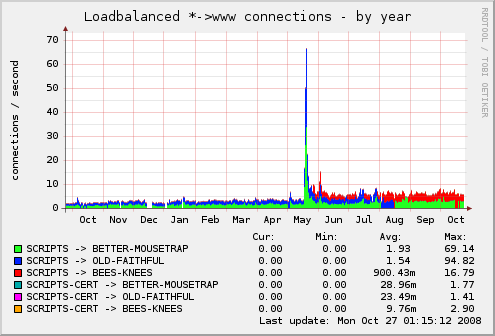
\includegraphics[width=3in] {Aggregated-cps_www-year.png}}
    \only<2>{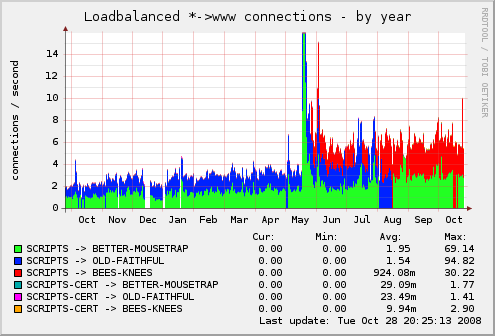
\includegraphics[width=3in] {Aggregated-cps_www-year-clip.png}}
  \end{center}
\end{frame}
